\section{Activation}
Before 2012, the logistic, the tanh and the pur linear functions where the standard activation functions, but then Alex Krizhevsky published an article where he introduced a new activation function called \textit{Rectified Linear Units (ReLU)} which outperformed the classical activation functions. [4] The network he used is now known as AlexNet, and helped to revolutionize the field of computer vision. [5] After that, the ReLU activation function has been modified several times (avoiding zero derivative among others), and example of innovations are \textit{leaky ReLU} and \textit{Exponential Linear Unit (ELU)}. All those networks are linear for positive numbers, and small for negative numbers. Often, especially in the output layer, a straight linear function is used as well.

In figure (\ref{fig:activation_functions}), \textit{standard RELU, leaky RELU} and \textit{ELU} are plotted along with the logistic function.

\iffalse
\begin{figure} [H]
	\centering
	\subfloat[logistic]{{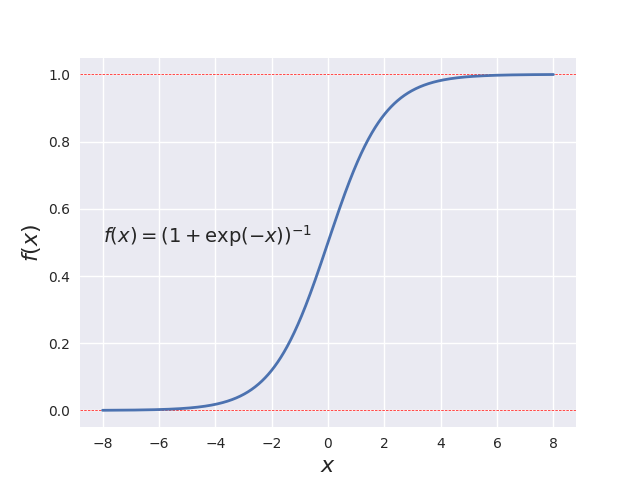
\includegraphics[width=8cm]{../plots/sigmoid.png} }}
	\subfloat[ReLU]{{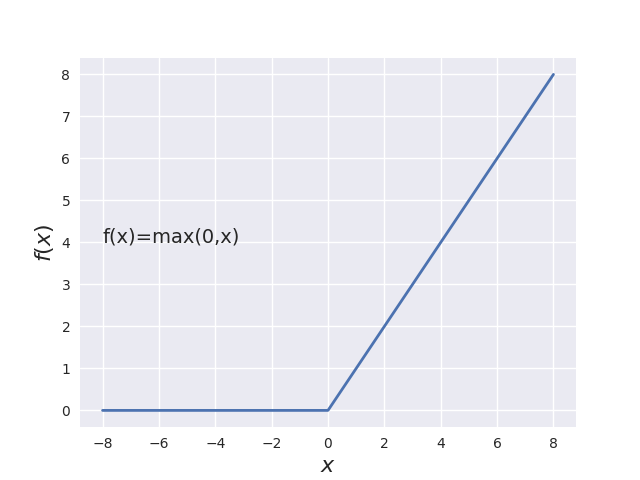
\includegraphics[width=8cm]{../plots/ReLU.png} }}\\
	
	\subfloat[Leaky ReLU]{{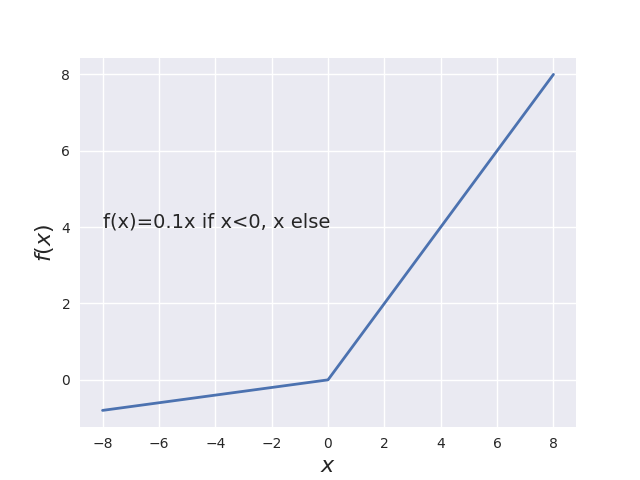
\includegraphics[width=8cm]{../plots/LeakyReLU.png} }}%
	\subfloat[ELU]{{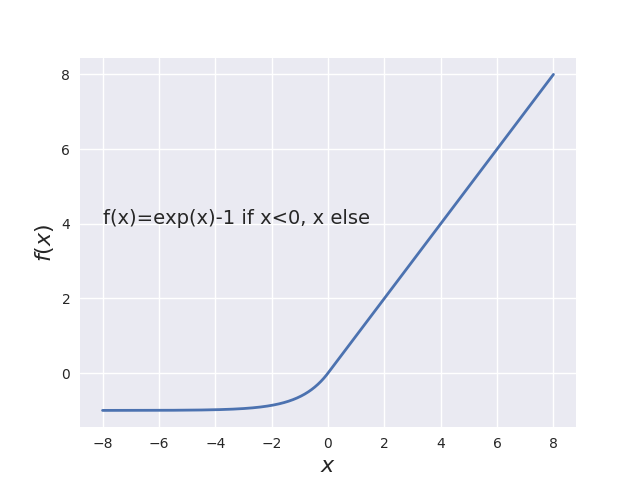
\includegraphics[width=8cm]{../plots/ELU.png} }}
	\caption{Some more or less popular activation functions}%
	\label{fig:activation_functions}%
\end{figure}
\fi

\subsection{Logistic}

\subsection{ReLU}

\subsection{ELU}